\chapter{引言}
\label{cha:intro}

\section{研究背景和研究意义}

\footnotetext[1]{Hadoop.~http://hadoop.apache.org/.}
\footnotetext[2]{Spark.~http://spark.apache.org/.}
\footnotetext[3]{Flume.~http://flume.apache.org/.}
\footnotetext[4]{Storm.~http://storm-project.net/.}
\footnotetext[5]{Ceph.~http://ceph.com.}
云计算技术是 IT 产业界的一场技术革命, 已经成为了IT行业发展的一个大方向。 
各国政府纷纷将云计算服务视为国家软件产业发展的新机遇。 
美国政府在IT政策和战略中也加入了云计算因素,美国国防信息系统部门 (DISA) 正在其数据中心内部搭建云环境\cite{fang-cloud}。
作为云计算的承载体-数据中心,近些年也受到了越来越多的关注。
事实上,从2010年起 , 全球数据中心的市场规模一年比一年庞大,
已经从2010年的20亿美元提高到了2015年的46亿美元,平均每年增长幅度达到了$14.3\%$\cite{wu-datacenter}。
所谓数据中心,就是一套由计算机及相关配套设备所组成的,
以储存、传递、展示、加工处理数据为主要目的的完善系统工程\cite{wu-datacenter}。
现在很多应用都部署在数据中心,为用户提供各种各样的服务,
例如,为用户提供计算服务的Hadoop \footnotemark[1]、Spark \footnotemark[2]、Flume \footnotemark[3]、Storm \footnotemark[4]等,为用户提供存储的ceph \footnotemark[5]等。
甚至,很多企业比如国外的facebook、youtube,国内的中国银行、中国电信等,都有自己的数据中心。
数据中心已经成为国内国外工业界和学术界关注的重心和研究热点。

在实际中,数据中心有成千上万台机器。
根据统计,截止2016年,
谷歌的数据中心中有多达45万台机器\cite{wei-dc}。
在数据中心的服务器中,部署着各种各样的应用,因为单个机器的
计算能力,容量等有限,而具有超高计算能力和超高存储能力的大型计算机的成本又太高,
因此,应用往往采取分布式的方法部署在集群中。
部署在集群中的应用数据流组,有共同的目标和共同的语义,
它们或是为了计算同一个目标,
或者是为了存储同一个巨型文件,
或者是为了达到同一个优化目标等。
各种各样的分布式应用部署在数据中心,
突出了数据中心作为信息服务载体的核心地位,
也同时给数据中心的建设提出了更加严峻的挑战。


数据中心网络(Data Center Networks,简称 DCNs)是指数据中心内部通过高速链路和交换机、路由器连接大量服务器的网络。
传统数据中心网络主要采用层次结构实现,
且承载的主要是客户机/服务器模式的应用。
多种应用同时在同一个数据中心内运行,每种应用一般运行在特定的服务器/虚拟服务器集合上\cite{wei-dc}。
数据中心的应用常常分布式的部署在集群中,
这些应用常常需要多个计算或者存储步骤才能得到预期的结果。
数据中心应用内部,应用之间往往进行频繁的通信,
数据中心网络,就是这些应用通信的桥梁。
随着数据中心规模的变大,
应用对数据中心网络提出了越来越高的要求,
网络性能已经逐渐成为数据中心发展的瓶颈。
在网络给数据中心提供的服务中,
应用获得的带宽和传输的延迟,是评价服务质量高低重要的因素,
它们对用户体验产生重要的影响。
甚至根据facebook的报告\cite{Latency},应用延迟每增加100毫秒,企业收入会减少1$\%$。


当前,越来越多的应用尤其是分布式应用部署在规模日益增大的数据中心集群中。
这些分布式应用常常有许多并行的数据流,
数据传输需要在一定截止期限(deadline)之前完成,否则会影响应用的性能。
例如分区-聚合(Partition-Aggregate)应用
要求叶节点的询问和应答传输在截止期限(deadline)之前完成。
任何没有在截止期限之前完成的数据流都被认定错失期限。
错失期限的数据流越多,会有越多的上层计算节点获得不完整的结果,进而影响服务的质量。
此外,在实际中不同的应用的数据流有不同的截止期限,
甚至,同一个应用的不同阶段的传输的期限也不相同。
此外,在数据中心内,有多阶段的分布式应用,对于多阶段的分布式应用,每个阶段存在一组并行数据流,
当组内所有数据流传输完成才能进入下一阶段。




这给数据中心网络带来了各种各样的问题和挑战,
如何合理的分配数据中心网络资源,
使得数据中心网络能够满足应用日益增加的需求,
是当前业界面临的一个重大挑战。
越来越多的研究集中在优化数据中心应用的传输带宽和延迟上。
互联网采用TCP作为传输协议,
但直接在数据中心采用TCP会导致一系列问题:
首先,TCP采取滑动窗口机制进行控制,
当发生拥塞时,交换机会出现丢包,此时发送端的拥塞窗口会减半,从而降低发送端速率。
此外,滑动窗口减半会导致链路利用率低。
没有拥塞时,发送端的拥塞窗口会不断增大,发送端速率不断增大,当并行的发送端较多时,会导致交换机缓冲区不断变大,引起较大的排队延迟。
此外,TCP是一种公平分配带宽的策略,然而对于数据中心的应用而言,不同的应用对延迟和带宽的需求是不同,
如时钟同步,Memcached,Naiad等应用需要数据中心网络提供低延迟,
而hadoop等计算应用需要数据中心网络提供高带宽。
事实上,数据中心的资源总量是一定的,
采用TCP进行传输,不能有效的满足应用对延迟和带宽的需求,
造成数据中心网络资源不能合理高效的使用,
因此,许多新型传输策略被提出。根据新型的网络传输协议的传输粒度,可以分成流级别的传输优化策略和任务级别的传输优化策略。


尽管当前的新型传输策略可以提升数据中心网络的传输性能,但是这些策略依然有很多不足。
首先,对于流级别的传输优化方案,无论是优化有期限的流还是优化流平均传输时间,
都没有考虑拥塞程度和流带宽之间的关系,导致在重度拥塞时不同期限的流获得带宽基本相同,不再基于期限进行带宽区分。
其次,当前流级别传输方案,都侧重单独解决期限问题或者优化短流延迟,
而并没有同时对二者优化。
此外,任务级别的传输调度,大多数根据网络情形优化任务的平均完成时间,而并未结合任务重要
性对任务进行调度,导致网络资源并没有合理的分配。


针对上述的问题,本文的研究意义在于,
首先构建基于应用的数据中心传输调度框架,为应用提供更好的用户体验。
其次对数据中心流和任务进行调度和传输优化,提高网络资源利用率。
本文的工作重点是:一是从流级别进行传输优化,改进数据传输协议,
根据网络拥塞状况和应用的期限等因子调整带宽,
进而提升应用的性能,提高用户体验。
二是从任务级别进行传输优化,进行任务级别调度。
通过给数据中心任务分配优先级,根据网络拥塞和应用优先级进行调度,
从而更合理的利用网络资源。
需要说明的是,本文提供的方法,不仅用于数据中心网络,
也可以用于其他类似网络环境。

\section{论文研究内容}
作者的博士论文主要包括以下几个方面:

\textbf{(1)~综述了国内外研究现状}

本文介绍数据中心应用传输方案的相关工作。
首先,从常见应用的通信模型和数据流量等方面对数据中心传输进行概述。
本文重点介绍4类通信模型:映射规约(Map-Reduce)模型,数据流(Dataflow)模型,整体同步并行计算(Bulk Synchronous Parallel)模型,
分区-聚合(Partition-Aggregate)模型,并介绍了短流、
长流等流量特征和数据中心应用期限等特征。
从流级别和任务级别综述并且分析了当前数据中心传输优化策略存在的不足,
发现无论是流级别传输还是任务级别传输都有很大的提升空间。

\textbf{(2)~研究了基于ECN标记的流传输模型}

本文提出了基于ECN标记的流模型。
首先,对基于ECN标记的流模型的场景进行介绍。
然后,介绍了基于ECN标记的流模型。
随后,使用基于ECN标记的流模型对LPD和FDRC策略进行参数分析,
并对基于ns-2的仿真结果和流模型推算结果进行对比,
同时指导LPD和FDRC关键参数的设置。

\textbf{(3)~研究了基于负载自适应原则的传输优化方案 }

本文主张在设计数据流传输方案时,
应该遵循一个简单的原则:
拥有不同截止期限的流在其带宽分配和占用上应该被区分,
网络负载越重,数据流越被区分。
本文认为设计流量控制策略时应该遵循这个原则。
基于这个原则,本文并提出了一种简单的拥塞控制算法-正比负载差分
(Load Proportional Differentiation,简称LPD)策略作为其应用。
在不同的仿真环境和测试床上,使用不同的网络拓扑和负载情况评估LPD的性能。

\textbf{(4)~研究了基于流持续时间的传输优化方案}

由于TCP不能满足应用程序对延迟和吞吐量的要求,因此业界提出了许多基于TCP的协议(例如,DCTCP,D$^2$TCP,L$^2$DCT)来对TCP进行补充。
其中D$^2$TCP等协议将明确的截止时间纳入拥塞窗口调整过程,以保证流在截止期限之前完成。
L$^2$DCT等协议在计算拥塞窗口调整因子时考虑流量大小,保证短流的吞吐量和延迟。
这两种方法在一定的场景下运行良好,但在两个方面存在一些不足。
首先,这两种方法只能减小流错失期限的百分比或者能够减小短流延迟,但是不能够同时优化这两个目标。
其次,这两种方法都需要用户得知流信息(例如截止时间,流量大小),对于一些应用来说,这些信息可能很难事先确切得知。
本文主张将流持续时间引入拥塞窗口调整的过程中。
基于此,本文提出基于流持续时间速率控制(Flow Duration Rate Control,简称FDRC)机制。
在无需知流具体信息的情况下,FDRC可以达到同时减少流错失期限的比例和减小流平均完成时间。
本文从理论上分析了FDRC的行为,并在ns-2和Linux内核实现和评估FDRC。

\textbf{(5)~研究了数据中心任务级传输优化模型}

本文提出了数据中心任务传输模型,介绍了数据中心非阻塞模型,
定义了数据中心传输任务和数据中心任务级传输优化问题的数学表达形式。
同时,针对数据中心任务级传输优化问题,分析了数据中心传输任务调度问题的复杂度。
提出了针对传输任务最小化平均延迟的离线调度算法,并证明数据中心任务级离线调度算法的近似度。

\textbf{(6)~研究了基于流信息的任务级传输优化方案 }

数据中心存在很多分布式应用,这些分布式应用每个阶段会传输一组并行的流,
当本阶段所有数据流均传输完毕时,才能够进行下一阶段计算和传输。
因此进行任务级别传输十分有必要。
本文提出了基于流信息的任务级传输优化方案,
预先得知每条流信息的前提下,在非阻塞模型的基础上,对传输任务进行传输优化。
同时,本文以纠删码存储系统为例,将纠删码选源和任务级传输结合一起进行优化,
大幅度提高了纠删码存储系统的文件传输效率。

\textbf{(7)~基于重要性和网络拥塞的任务传输调度方案}

传统的网络资源管理机制主要是流级别或者报文级别的。
最近,流组(coflow)作为对分布式应用传输任务的抽象模型而被提出。
通过将流组作为网络资源分配或调度的基本元素可以更好的实现一些高级优化目标,如减少应用平均传输延迟等。
虽然业界已经提出一系列流组调度方案,但是大多数方案并没有考虑应用的重要性,
这会导致重要应用无法获得应有的带宽,网络利用率低下的问题。
因此如何根据应用的重要性和网络拥塞程度对应用进行调度是一个重要问题。
本文测量数据中心应用流量的特性,
发现了当前流组调度策略Varys未考虑应用重要性,导致重要应用未获得足够带宽,性能受到影响的问题,并且分析此问题。
提出基于流组重要性和网络拥塞程度进行任务传输调度的方案,
同时使用真实的数据中心流量对在线调度策略进行评估。


\textbf{(8)~设计实现和评估了数据中心应用传输优化系统}

本文设计并实现了数据中心传输系统 FlyTransfer,架构和系统的各个组件。
随后使用了数据中心真实流量,从任务级别调度,流级别优化和系统开销等方面对系统进行了性能评估。

\section{论文的主要贡献}
\textbf{(1)提出了基于负载自适应原则的传输优化方案}

针对数据中心流级别传输方案在重度拥塞时失效的问题,
本文主张在设计基于期限的流传输方案时,
应该遵循一个简单的原则:
拥有不同截止期限的流在其带宽分配和占用上应该被区分开,
且网络负载越重,数据流越被区分。
设计流量控制策略时应该遵循这个原则。
基于此原则,本文提出了一种简单的拥塞控制算法-正比负载差分
(Load Proportional Differentiation,简称LPD)策略作为其应用。
当网络负载严重时,在预先得知流信息前提下,LPD依然可以根据数据流期限进行速率控制。
本文在不同的网络拓扑和网络负载的场景下评估LPD。

\textbf{(2)提出了基于流持续时间的传输优化方案}

针对当前数据中心流级别传输优化策略,或者优化有期限的流,
或者优化短流传输延迟,并未对二者同时进行优化的问题,
本文主张引入流持续时间进入拥塞窗口调整的过程中,
同时提出基于流持续时间速率控制机制(Flow Duration Rate Control,简称FDRC)。
在无需得知流信息的前提下,FDRC可以同时减少流错失期限的比例并且减小流平均完成时间。
本文从理论上分析了FDRC的性能,并在ns-2和Linux内核实现FDRC。
实验表明,在几乎所有场景下,FDRC性能优于D$^2$TCP和L$^2$DCT。



\textbf{(3)提出了基于流信息的任务级传输优化方案}

针对分布式应用进行流级别传输不一定能满足应用对带宽的需求的问题,
本文提出需要对数据中心应用进行任务级传输优化,
并在非阻塞模型下提出数据中心任务传输的2-近似离线策略。
同时结合最小负载优先的启发式的数据源的选择策略,
对纠删码存储系统进行最小化文件平均访问时间(File Access Time,简称FAT)的优化。
在此基础上,本文设计并实现了D-Target,并使用AT\&T的纠删码数据评估D-Target的性能。

\textbf{(4)提出了基于重要性和网络拥塞的任务传输调度方案}

针对当前数据中心对应用的传输,只考虑网络拥塞,并未考虑应用重要性的问题,
本文提出使用权重代表应用重要性,进行加权流组完成时间(Weighted Coflow Completion Time,简称WCCT)最小化问题的优化。
针对此问题,本文设计了无需预先得知流大小就可以进行传输任务调度的在线算法-Yosemite。
Yosemite可以根据流组权重和网络拥塞程度进行任务级别调度,
本文同时使用数据中心的真实流量对在线算法Yosemite进行评估。


\section{论文的组织结构}
\label{cha:LPD}
\begin{figure}[b]
\begin{center}
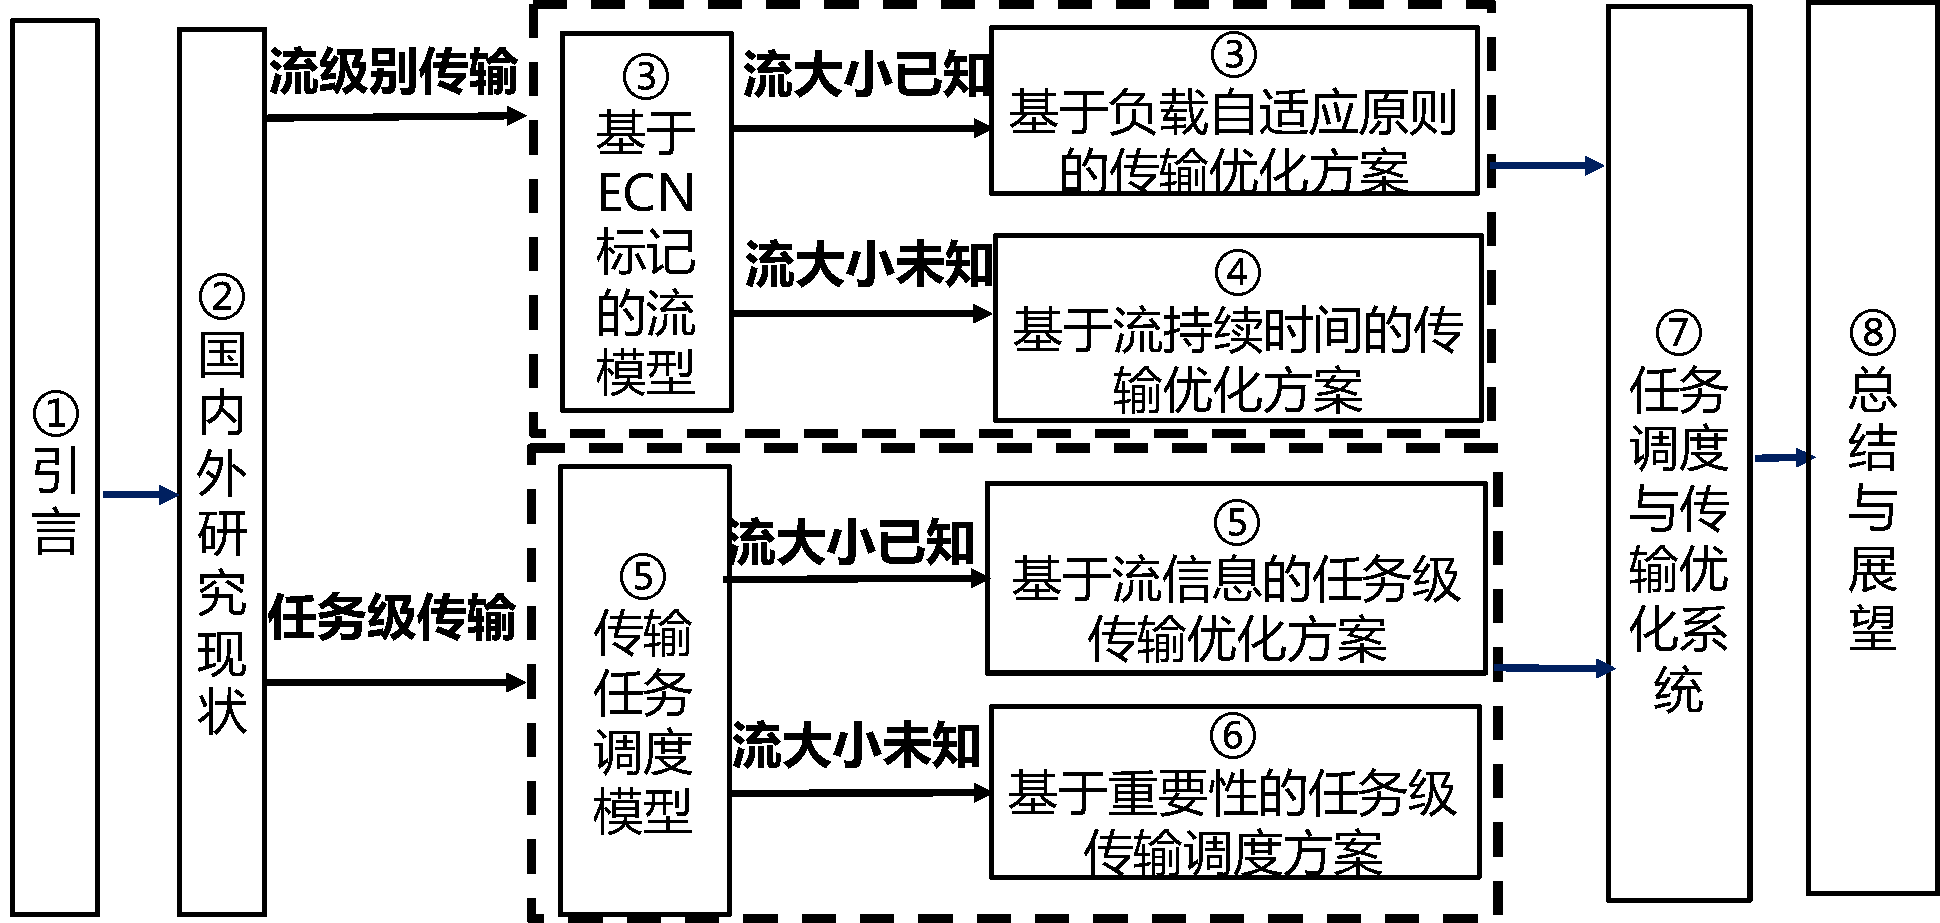
\includegraphics [width=0.9\columnwidth] {figures/structure.pdf}
\caption{论文结构}
\label{paper-structure-fig}
\end{center}
\end{figure}
如图\ref{paper-structure-fig}所示,本文总共分为8章,其中,本章(第1章)是论文引言部分,第2章到第7章是论文的主体部分,
包括流级别的传输优化,任务级别的传输优化和应用传输系统的介绍。
论文的第3章和第4章侧重流级别的传输优化,
第3章介绍了基于 ECN 标记的流模型,
并且提出了基于负载自适应原则的传输优化方案。
第4章介绍了基于流持续时间的传输优化方案。
论文的第5章和第6章介绍的是任务级传输优化方法。
其中第5章介绍了传输任务调度模型,并提出基于流信息的任务级传输优化方案。
第6章介绍了基于重要性的任务级传输调度方案。
第7章主要介绍应用传输系统FlyTransfer以及其性能评测。
第8章是论文的总结部分,主要是对当前工作的总结和对未来工作的展望。


